\begin{figure*}[htbp!]
\centering
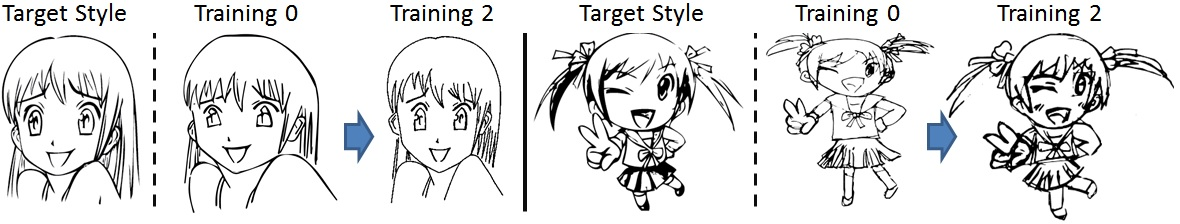
\includegraphics[width = 1.0\textwidth]{images/trainingSamples}
\vspace{-4mm}\caption {Samples sketches drawn by artists at the first and final stages of training along with the target style sketches. Sketches on the left correspond to the intermediate artist while ones on the right to the novice artist. The progress in their sketching styles is noticeable for both artists but more so for the novice one.}
\label{trainingSamples}\vspace{-4mm}
\end{figure*}

In this section, we show SAR's feasibility in two useful applications other than sketch fraud detection, namely sketch style training and sketch synthesis evaluation.

%various applications that require the comparison between artists' sketching styles (e.g. fraud detection and teaching artistic style).

\vspace{-2mm}
\subsection{SAR for Sketch Style Training}
\vspace{-2mm}
Knowing that an artist's sketching style is dynamic (i.e. it evolves over time), how persistent is it when artists undergo extensive training for the explicit purpose of altering their style and adopting another? For example, this type of training is administered in major cartoon companies (e.g. Walt Disney), usually for months on end. For this purpose, we develop a SAR-based application that allows artists, designers, and animators in-training to quantify their progress in adopting the \emph{target} style of a particular artist, whose sketches have been encoded in SAR. Trainees are able to draw and/or upload sketches to examine how close their artistic style has become to the target. We demonstrate this application next.

%%%%%%%%%%%%%%%%%%%%%
%% might want to re-add the fact that this same app can be used to show which artists have the same style and help them decide on which artists to work with.
%%%%%%%%%%%%%%%%%%%%%%


%For example, such an application can assist artists in deciding which artists to work with in group projects (based on high affinity values) or it can quantify how an artist-in-training is learning to draw with a particular sketching style. The later is what we are demonstrating next.

\textbf{Style Training Setup} We first determine a target style by finding a reasonably known artist, who has published his work online along with specific instructions on how to follow his drawing style. The target artist also provides YouTube videos showing how his sketches can be drawn step-by-step. We select fives sketches from his portfolio, specifically those with video instructions. Then, we identify three artists with varying levels of sketching and artistic experience (novice, intermediate, and advanced) to undergo the style training process. The advanced level artist is a professional with 10 years of experience and the intermediate artist has 3, while the novice artist only sketches as a hobby.

In the first stage of training, we ask all three artists to draw the five target sketches and then use the SAR-based tool to give them quantitative feedback on how similar their sketching style is to the target. The measure based on BoW features defined earlier in Section \ref{subsec:variations} is used to compute style similarity. In the second stage, we ask the artists to draw the sketches again after consulting a set of textual instructions on how to draw the target sketches. These instructions are obtained from the target artist's website. In the third stage, we provide the artists with their new SAR similarity scores along with instructional online videos. After submitting their newest sketches, we again compute their SAR similarity scores. Sample sketches of both novice and intermediate level artists at the first and last stages of training are shown in Figure \ref{trainingSamples}. It is obvious from these results that the novice artist has improved more significantly than the intermediate artist in adopting the target style.

%We first chose a set of 5 sketches drawn by one artist whose work is published over the internet with specific instructions on how to draw his sketches and how to follow his style. This is along with videos where the artist draws these set of sketches in step-by-step manner.

%After that, we trained SAR's application on these set of sketches. Next, we picked 3 artists such that each have a different sketching experience level. The first one is a novice artist with a minimum drawing experience while the second has an intermediate sketching level skills with only 3 years of practice and the third is an artist by profession with 10 years drawing experience.

%In the first stage of the training, we asked them to draw the chosen sketches and then use SAR to give them feedback on how their sketching style is close to the assigned sketches. In the second stage, we assigned them  the same sketches along with SAR's closure \% results and a set of instructions on how to draw the given sketches with that particular artistic style. We took those instructions from the website of that artist. In the third stage we provided them with a new SAR's closure \% results and videos on how to draw these specific sketches. Finally, we provided the participating artists with a SAR's closure \% which reflects how artists managed to modify their sketching style to match another artistic style. The training sketches used in this application at the 3 different will publicly be made available to allow for further testing and experimenting. Sample sketches of both novice and advanced level artists which visually shows how artists have evolved in their sketching styles is shown in Figure \ref{trainingSamples}.


\textbf{Style Training Results} Figure \ref{TrainingProgress} plots the evolution of the SAR similarity score throughout the 3-stage training process for each artist. As expected, each trainee's score increases with training. The novice artist exhibits an overall improvement of 10\%, which can be attributed to the explicit use of textual and video instruction for target training. The initial similarity scores for the intermediate and advanced level artists are much higher than the novice one, but they also exhibit an improvement of 4\% and 2\% respectively. The slight improvement by the advanced artist conveys how difficult it is for an artist with a well-defined style and extensive experience to adopt a new style, as well as, how much easier it is for a novice artist to do the same. Moreover, we expect that repeating these training stages (especially the last one) will further improve SAR similarity to the target style. Based on our results, we conclude that SAR can be successfully incorporated in the sketch training process (e.g. in major cartoon companies) to quantitatively monitor training progress. A training executable is available in the \noindent{\bf supplementary material}. We will also release the training source code to extend this application to a larger set of sketches from more participating artists and to allow users to build their own training applications using their own sketch data.


%progress in approaching the style of the assigned set of sketches while intermediate level artist progressed by 4\%. Advanced artist, on the other hand, progressed with only 2\%. Closure results as proposed by SAR at the 3 different stages of the training is shown in Figure \ref{TrainingProgress}.

%This difference in progress \% between novice and advanced artists conveys how it is difficult for an artist with well defined style and long experience to draw with a new style while novice artists have higher ability to learn new styles. \SARA {In addition, advanced and intermediate artists have initially drawn the sketches in the first training stages with higher closure \% than novice artist.}




%The target sketches used in this application will be made publicly available to allow for further testing and experimentation.



%%%%%%%%%%%%%%%%%%%%%%%%%%%
%% add as future work: we want to develop a system that will suggest possible changes to the strokes in a sketch to become more like the target style
%%%%%%%%%%%%%%%%%%%%%%%%%%%

%Old Application: To this end, we present a straightforward application that demonstrates a training program that allows artists, designers, and animators to quantify their affinity to any given artist, whose sketches have been incorporated in training SAR. Users are able to draw or upload their sketches and examine how close their artistic style is to the pre-defined artists from  the different datasets included in this paper (refer to Section \ref{sec:datasets}). The executable of our application is available in the \noindent{\bf supplementary material}. For example, such an application can assist artists in deciding which artists to work with in group projects (based on high affinity values) or it can quantify how an artist-in-training is learning to draw with a particular sketching style as illustrated in \ref{training}. We aim to extend this application to a larger set of sketches from more participating artists and to allow users to build their own SAR classifiers on their own datasets by releasing the training source code.

%The answer to this question can be empirically verified by estimating SAR accuracy throughout the extent of the training period. We expect this accuracy

\vspace{-3mm}
\begin{figure}[ht]
\centering
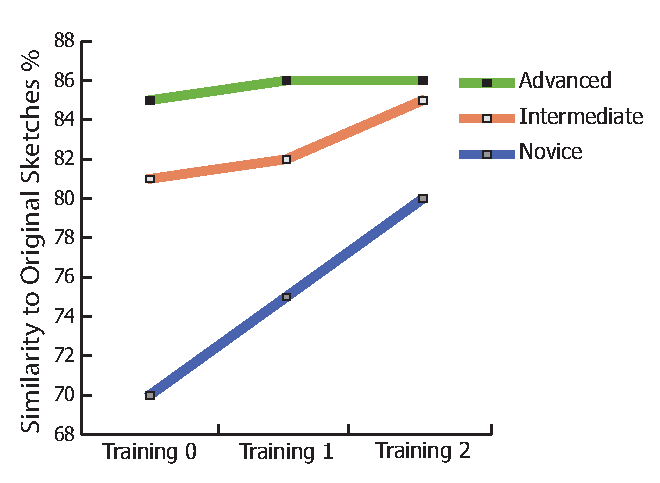
\includegraphics[width = 0.45\textwidth]{images/TrainingProgress}
\vspace{-2mm}\caption {SAR similarity-to-target scores for 3 novice, intermediate, and advanced level artists after 3 stages of training. The novice artist has the least score in the initial stage but progresses the most with training.}
\label{TrainingProgress} \vspace{-1mm}
\end{figure}


%\B{Change y-label to "Similarity to Target Style"}

\vspace{-2mm}
\subsection{SAR for Evaluating Sketch Synthesis Results}
\vspace{-2mm}
As mentioned in Section \ref{subsec: artisticanalysis}, there is a number of recent methods that focus on sketch synthesis and artistic style analysis. Their aim is to develop automatic sketch synthesis tools that mimic a particular artistic style. Most of these tools do not provide a quantitative assessment of how close the synthesized style is to the target one, thus, making it difficult to compare synthesis methods. A few of them however have validated their synthesis quality through extensive user studies, which are cumbersome to compile and require careful analysis. Since SAR is fully automatic, easy to use, and has proven style discrimination power (refer to Section \ref{subsec:recognition}), we propose to use it in quantitatively evaluating sketch synthesis methods without the need to conduct tedious user studies. To exemplify this application, we use SAR to analyze the synthesis results of Berger et. al. \shortcite{Berger:2013:SAP:2461912.2461964}. In their work, portrait sketches are synthesized from artistic styles of 7 artists, each of which drew 24 portrait sketches. The real and synthesized sketches are publicly available.


%A random choice classifier in this case has an average accuracy of 14\%.


We first use SAR to classify artistic style among the real portrait sketches only. In this case, SAR accuracy is 52\% (leave-one-out) and 50\% (5-fold), as compared to random chance accuracy of 14\%. When classifying only synthesized sketches, we obtain 54\% accuracy (leave-one out) and 51\% accuracy (5-fold) respectively. The  similarity in performance between the two scenarios suggests that the synthesized portraits are as hard to distinguish as the real ones and that the synthesis tool of \cite{Berger:2013:SAP:2461912.2461964} maintains a very similar amount of style diversity as in the real sketches. Next, we use SAR to classify the real sketches using the synthesized ones only as training and vice versa. In this case, SAR accuracy dropped to 26\% (leave-one-out) and 25\% (5-fold). This performance \emph{drop} can be used as a quantitative measure of synthesis quality, as it allows for comparison between different synthesis methods. In fact, an ideal synthesis tool should produce a SAR accuracy drop close to zero, since the style of the synthesized sketches should be undistinguishable from that of the real sketches.

Our results are on par with those of the three user (perceptual) studies conducted by Berger et. al. \shortcite{Berger:2013:SAP:2461912.2461964}. In fact, we setup the SAR classification experiments above to follow the same setup used in these user studies, where the only difference between the two is that SAR performs the classification automatically without any human feedback. The participants in the user studies registered a very similar accuracy when classifying the real and synthesized portraits separately (as did SAR). More importantly, the drop in classification by human participants is around 20\%, which is comparable to the 25\% drop reported by SAR. This result validates that SAR can be used to automatically and quantitatively evaluate sketch synthesis tools, without the need for user studies.


%To assess their synthesized results, they conduct 3 user studies involving 20 participants. In the first study, they asked participants to match a query real sketch to the artist they think drew it based on samples of real sketches of each artist. The second study, on the other hand, was the same but synthesized sketches were given in the query and in the provided samples. Participants registered similar accuracy in both studies which is aligned with our automated results shown above regardless of the fact that human performance was overall higher. In the third study, they asked participants to classify synthesized sketches to a collection of real sketches and vice versa. Participants performance dropped down by around 20\% compared to the first 2 studies which is the same amount of drop obtained by SAR. Their user studies provided us with a reliable baseline to assess SAR accuracy results.

%\textbf{Evaluation}
%Berrge et. al. \shortcite{Berger:2013:SAP:2461912.2461964} have conducted similar user studies to assess their synthesize results which involved a total of 20 adults and simulates a leave-one out cross validation scenario. Our automated results are aligned with their perceptual study results as follows: In classifying synthesize and real sketches separately, participants were 76.4\% and 72.4\% accurate respectively. SAR automated results, on the other hand was almost 20\% less but consistent with the user study results in terms of the minimum differences between classifying real and synthesized sketches.

%In another study, they asked participants to classify synthesized sketches to a collection
%of real sketches and vice versa. Participants performance dropped to 48\% and 50\%. Accuracy results of SAR went down by the same amount to become 25\%.

%This shows how challenging it is to build an accurate automatic replication of an artist's style as explained by the differences in the results above for both SAR and the user study they provided.

%. However, this was not the case in the portrait sketch dataset as the classification accuracy dropped down to 25\%.


%In this section we present an application that we built by utilizing the best performing computational model described in the previous sections. It makes use of all the different datasets provided in this work. Our application spots the light on one of the areas in which SAR can serve and that is analysis of artistic styles among different artists.

%We demonstrate a training program that allows artists, designers and animators to test their affinity to any given artist, whose works have been incorporated into the machine learning part of the program. Users are able to draw or upload their sketches and examine how close their artistic style to our defined artists who participated in creating the different datasets provided in this paper. Such application can for example assist artists to decide with which artists to work with in group projects or It can assess how an artist's style is approaching another style over training. We hope to see an extension of our application using a variety of artists sketches examples. The executable of our application is available in the \noindent{\bf supplementary material.}
